\section{Burger's Equation}
In this problem you will solve Burgers equation, $u_t+f_x= 0,\ f=\frac{1}{2}u^2,\ x \in [0,4)$, periodic boundaries, with the initial condition shown below.

\begin{figure}[h]
    \centering
    

\tikzset{every picture/.style={line width=0.75pt}} %set default line width to 0.75pt        

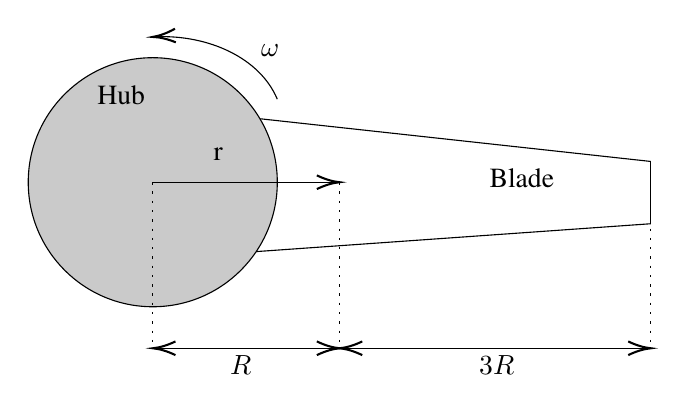
\begin{tikzpicture}[x=0.75pt,y=0.75pt,yscale=-1,xscale=1]
%uncomment if require: \path (0,300); %set diagram left start at 0, and has height of 300

%Shape: Circle [id:dp6244430308199536] 
\draw  [fill={rgb, 255:red, 202; green, 202; blue, 202 }  ,fill opacity=1 ] (220,120) .. controls (220,86.86) and (246.86,60) .. (280,60) .. controls (313.14,60) and (340,86.86) .. (340,120) .. controls (340,153.14) and (313.14,180) .. (280,180) .. controls (246.86,180) and (220,153.14) .. (220,120) -- cycle ;
%Straight Lines [id:da1433381310737285] 
\draw    (520,110) -- (520,140) ;
%Straight Lines [id:da6958270078143212] 
\draw    (520,110) -- (331.79,89.43) ;
%Straight Lines [id:da5982890152434965] 
\draw    (520,140) -- (329.79,153.43) ;
%Straight Lines [id:da7103183675633375] 
\draw    (280,120) -- (368,120) ;
\draw [shift={(370,120)}, rotate = 180] [color={rgb, 255:red, 0; green, 0; blue, 0 }  ][line width=0.75]    (10.93,-3.29) .. controls (6.95,-1.4) and (3.31,-0.3) .. (0,0) .. controls (3.31,0.3) and (6.95,1.4) .. (10.93,3.29)   ;
%Straight Lines [id:da18697245418380692] 
\draw  [dash pattern={on 0.84pt off 2.51pt}]  (280,120) -- (280,200) ;
%Straight Lines [id:da9445115873305969] 
\draw  [dash pattern={on 0.84pt off 2.51pt}]  (370,120) -- (370,200) ;
%Straight Lines [id:da8681269156370801] 
\draw    (282,200) -- (368,200) ;
\draw [shift={(370,200)}, rotate = 180] [color={rgb, 255:red, 0; green, 0; blue, 0 }  ][line width=0.75]    (10.93,-3.29) .. controls (6.95,-1.4) and (3.31,-0.3) .. (0,0) .. controls (3.31,0.3) and (6.95,1.4) .. (10.93,3.29)   ;
\draw [shift={(280,200)}, rotate = 0] [color={rgb, 255:red, 0; green, 0; blue, 0 }  ][line width=0.75]    (10.93,-3.29) .. controls (6.95,-1.4) and (3.31,-0.3) .. (0,0) .. controls (3.31,0.3) and (6.95,1.4) .. (10.93,3.29)   ;
%Straight Lines [id:da9459156094037822] 
\draw    (372,200) -- (518,200) ;
\draw [shift={(520,200)}, rotate = 180] [color={rgb, 255:red, 0; green, 0; blue, 0 }  ][line width=0.75]    (10.93,-3.29) .. controls (6.95,-1.4) and (3.31,-0.3) .. (0,0) .. controls (3.31,0.3) and (6.95,1.4) .. (10.93,3.29)   ;
\draw [shift={(370,200)}, rotate = 0] [color={rgb, 255:red, 0; green, 0; blue, 0 }  ][line width=0.75]    (10.93,-3.29) .. controls (6.95,-1.4) and (3.31,-0.3) .. (0,0) .. controls (3.31,0.3) and (6.95,1.4) .. (10.93,3.29)   ;
%Straight Lines [id:da5900923017563646] 
\draw  [dash pattern={on 0.84pt off 2.51pt}]  (520,120) -- (520,200) ;
%Curve Lines [id:da19047210809641868] 
\draw    (340,80) .. controls (331.57,59.94) and (306.65,48.98) .. (281.9,49.91) ;
\draw [shift={(280,50)}, rotate = 356.45] [color={rgb, 255:red, 0; green, 0; blue, 0 }  ][line width=0.75]    (10.93,-3.29) .. controls (6.95,-1.4) and (3.31,-0.3) .. (0,0) .. controls (3.31,0.3) and (6.95,1.4) .. (10.93,3.29)   ;

% Text Node
\draw (331,52.4) node [anchor=north west][inner sep=0.75pt]    {$\omega $};
% Text Node
\draw (316,202.4) node [anchor=north west][inner sep=0.75pt]    {$R$};
% Text Node
\draw (436,202.4) node [anchor=north west][inner sep=0.75pt]    {$3R$};
% Text Node
\draw (252,72) node [anchor=north west][inner sep=0.75pt]   [align=left] {{\fontfamily{ptm}\selectfont Hub}};
% Text Node
\draw (441,112) node [anchor=north west][inner sep=0.75pt]   [align=left] {{\fontfamily{ptm}\selectfont Blade}};
% Text Node
\draw (308,102) node [anchor=north west][inner sep=0.75pt]   [align=left] {{\fontfamily{ptm}\selectfont r}};


\end{tikzpicture}

    \caption{Initial condition to Burgers equation.}
\end{figure}

For the numerical method, use the finite volume method (FVM) with $N_x$ uniform cells, forward Euler time stepping, a uniform time step, CFL=0.8 (based on the initial condition), and the upwind flux,

\begin{equation*}
    \hat{F}_{j + \frac{1}{2}} = \frac{1}{2}\left(f_j + f_{j+1}\right) - \frac{1}{2}|\hat{a}_{j + \frac{1}{2}}|\left(u_{j+1} - u_j\right)
\end{equation*}

\begin{enumerate}[label=\alph*., start = 1]
    \item Prior to implementing the FVM, determine the analytical solution using the method of characteristics. Plot the state, $u(x,t)$, at times $t= 0.5,\ 1.0,\ 1.5$ in one figure. In a separate figure, make a space-time diagram of the characteristics, up to $t= 1.5$, and indicate any shock speeds/paths.

    \vspace{-0.25in}
    \begin{align*}
        \shortintertext{Firstly, to start out numbering the regions. Region 1 will be from $0\rightarrow 1$, Region 2 from $1\rightarrow 2$, Region 3 from $2\rightarrow 3$, Region 4 from $3\rightarrow 4$. This gives,}
        \textbf{Region 1:}\quad & u(x,0) = 0\quad \forall\ x \in [0, 1)\\
        \textbf{Region 2:}\quad & u(x,0) = x-1\quad \forall\ x \in [1, 2)\\
        \textbf{Region 3:}\quad & u(x,0) = 3-x\quad \forall\ x \in [2, 3)\\
        \textbf{Region 4:}\quad & u(x,0) = 0\quad \forall\ x \in [3, 4)\\
        \shortintertext{This gives that the Initial condition can be expressed as}
    \end{align*}

    \vspace{-0.45in}
    \begin{equation*}
        u(x,t=0) = \begin{cases}
            0 & x \in [0,1]\\
            x - 1 & x \in [1,2]\\ 
            3-x & x \in [2,3]\\ 
            0 & x \in [3, 4]
        \end{cases}
    \end{equation*}

    \vfill 
    Continued on the next page \ldots 

\end{enumerate}


\pagebreak
\pagestyle{fancy}
\restoregeometry
\begin{adjustwidth}{2.5em}{0pt}

    \begin{align*}
        \shortintertext{Then this gives that the solution to Burgers Equation is,}
        u(x,t) & = u_0(x - ut)\\ 
        \shortintertext{Where in Region 2, the expression can be given by,}
        \frac{dx}{dt} & = x_0 - 1\\ 
        x & = x_0 + t(x_0 - 1),\ x_0  = \frac{x+t}{1+t}\\
        \shortintertext{Then again for Region 3, the expression is given by,}
        \frac{dx}{dt} & = 3 - x_0\\ 
        x & = x_0 + t(3-x_0),\ x_0  = \frac{x-3t}{1-t}\\
        \shortintertext{Substituting back into the final cases for the characteristics and equations gives,}
    \end{align*}

    \vspace{-0.5in}
    \begin{equation*}
        \boxed{u(x,t \le 1) = \begin{cases}
            0 & x \in [0,1]\\
            \frac{x+t}{1+t} - 1 & x \in [1,2]\\ 
            3 - \frac{x-3t}{1-t} & x \in [2,3]\\ 
            0 & x \in [3, 4]
        \end{cases},\qquad \frac{dx}{dt} = \begin{cases}
            0 & x \in [0,1]\\
            x_0 + t(x_0 - 1) & x \in [1,2]\\ 
            x_0 + t(3-x_0) & x \in [2,3]\\ 
            0 & x \in [3, 4]
        \end{cases}}
    \end{equation*}

    \vspace{-0.25in}
    \begin{align*}
        \shortintertext{Then, for the case when a shock forms,}
        s & = \frac{dx_s}{dt} = \frac{1}{2}(u_l + \cancelto{0}{u_r}) = \frac{1}{2}\left(\frac{x+t}{1+t} - 1\right)\\ 
        \shortintertext{Then performing a simple differential equatoin with the initial condition $x_s(1)=3$, when the shock forms gives that the expression for the shocks location is,}
        x_s & = 1 + \sqrt{2 + 2t}\\ 
        \shortintertext{At this moment the right side of the shock will zero or $u_r=0$, so then then at times higher than the shock forms the expression is then}
    \end{align*}

    \vspace{-0.35in}
    \begin{equation*}
        \boxed{u(x, t> 1) = \begin{cases}
            0 & x \in [0,1]\\
            \frac{x+t}{1+t} - 1 & x \in [1,1+\sqrt{2+2t}]\\ 
            0 & x \in [1+\sqrt{2+2t}, 4]
        \end{cases},\qquad \frac{dx_s}{dt} = \begin{cases}
            0 & x \in [0,1]\\
            \frac{1}{2}\left(\frac{x+t}{1+t} - 1\right) & x \in [1,1+\sqrt{2+2t}]\\ 
            0 & x \in [1+\sqrt{2+2t}, 4]
        \end{cases}}
    \end{equation*}

    \vfill 
    Continued on the next page \ldots 
    
\end{adjustwidth}

\pagebreak

\begin{adjustwidth}{2.5em}{0pt}
    Plotting the characteristics, and the state gives the following results,

    \begin{figure}[h]
        \centering
        \begin{subfigure}[b]{0.45\linewidth}
            \centering
            \includegraphics[width = \linewidth]{q1/analytical.pdf}
            \caption{Analytical expression for Burgers equation at varying times.}
            \label{fig:analytical}
        \end{subfigure}
        \begin{subfigure}[b]{0.45\linewidth}
            \centering
            \includegraphics[width = \linewidth]{q1/characteristics.pdf}
            \caption{Characteristics of the initial condition of the Burgers equation.}
            \label{fig:characteristics}
        \end{subfigure}
        \caption{Plots of the analytical Burgers equation and its characteristics at varying times $t$.}
        \label{fig:combined_analytical_characteristics}
    \end{figure}

    \begin{fminipage}{0.9\linewidth}
        \textbf{As shown above in Figures \ref{fig:analytical}, \ref{fig:characteristics} are the implementations of the analytical solution and the characteristics in Python. Shown above in \ref{fig:analytical} is the actual shock paths as the time varies. At time $\bf t=1$, the shock first forms the discontinuity. Denoted in Figure \ref{fig:characteristics} by the black line is the shock path following the line $\bf x_s = 1+\sqrt{2 + 2t}$ for times greater than ``1'' after the shock forms.}
    \end{fminipage}
\end{adjustwidth}


\pagebreak    
\begin{enumerate}[label=\alph*., start = 2]
    \item Implement the FVM and using $N_x$= 128 and $N_x$= 512, show the states at the same times as requested in the previous part. Make three plots, one for each time, and overlay the two $N_x$ results and the analytical solution on each plot. Comment on the differences.
    
    \vspace{-0.15in}
    \begin{figure}[h!]
        \centering
        \begin{subfigure}[h]{0.7\linewidth}
            \centering
            \includegraphics[width = \linewidth]{q1/t05.pdf}
            \caption{Burgers equation approximated solutions at time $t=0.5$ for $N_x=128,\ N_x =512$.}
            \label{fig:q1_t05}
        \end{subfigure}
        \begin{subfigure}[h]{0.7\linewidth}
            \centering
            \includegraphics[width = \linewidth]{q1/t10.pdf}
            \caption{Burgers equation approximated solutions at time $t=1.0$ for $N_x=128,\ N_x =512$.}
            \label{fig:q1_t10}
        \end{subfigure}
        \begin{subfigure}[h]{0.7\linewidth}
            \centering
            \includegraphics[width = \linewidth]{q1/t15.pdf}
            \caption{Burgers equation approximated solutions at time $t=1.5$ for $N_x=128,\ N_x =512$.}
            \label{fig:q1_t15}
        \end{subfigure}
        \caption{Implementation of the Finite Volume Method (FVM) at varying times.}
        \label{fig:q1_shocks}
    \end{figure}

    \begin{fminipage}{0.8\linewidth}
        \textbf{Shown above in Figure \ref{fig:q1_shocks} is the approximated solution to Burgers equation and the forming shock. Uniform across all the times, is that at a higher $\bf N_x$ value there is a better approximation to analytical solution. Shown best in Figure \ref{fig:q1_t10} is how the approximated finite volume method bends around the shock arising from the weak solution.}
    \end{fminipage}
\end{enumerate}
    
\pagebreak
\begin{enumerate}[label=\alph*., start = 3]
    \item Perform a convergence study of the FVM, using the $L_2$ solution error norm at $t = 0.5$, for $N_x= 128,\ 256,\ 512,\ 1024.$  Include an error convergence plot and compute/discuss the rate.
    
    \begin{figure}[h]
        \centering
        \includegraphics[width = 0.9\linewidth]{q1/convergence.pdf}
        \caption{Convergence studies for the finite volume method}
        \label{fig:q1_converge}
    \end{figure}

    \begin{fminipage}{0.8\linewidth}
        \textbf{Shown above in Figure \ref{fig:q1_converge} is the $\bf L_2$ solution error norm for the finite volume method. As shown in the figure, this implementation has a convergence of $\bf \approx \mathcal{O}(1)$ indicating that it is first-order accurate. Shown below in Table \ref{tab:q1_convergences} are the converge rates at each interval stepping to the next confirming first-order accuracy.}
    \end{fminipage}


    \begin{table}[h]
        \centering
        \caption{Convergence rates for the finite volume method.}
        \label{tab:q1_convergences}
        \begin{tabular}{l | l}
            Intervals & Rate\\\hline\hline
            \input{q1/convergences}
        \end{tabular}
    \end{table}
\end{enumerate}
